%Todos os resultados coletados e analisados neste artigo foram obtidos com base no consumo energético de dispositivos (nós) vestíveis sem fio produzidos pela empresa Shimmer~\cite{burns2010shimmer}, modelo 2R. Estes instrumentos proporcionam a coleta de sinais vitais de pacientes por meio de sensores, tais como acelerômetro, magnetômetro, giroscópio, entre outros. Após coletados, os sinais vitais devem ser transferidos para outros dispositivos computacionalmente mais eficientes, conhecidos como coordenadores da rede corporal sem fio. Esta transmissão pode ser realizada de dois modos. O primeiro modo ocorre de forma direta, utilizando-se a tecnologia Bluetooth. A outra maneira seria com o auxílio de dispositivos de retransmissão e para tal feito, a transferência é realizada utilizando rádio ZigBee, uma vez que proporcionam melhor eficiência energética.

The experiments in this letter rely on wearable devices from the Shimmer platform, model 2R. %, as illustrated in Figure~\ref{fig:Shimmer}. % illustrates the main experimental scenario. 
These devices sense vital signs and movements from users by accelerometers, magnetometers, and gyroscope, and transmit them to a coordinator device (e.g., a smartphone) through wireless communication, such as Bluetooth or Zigbee. These devices run the Real Time Operating System (RTOS) together to TinyOS. NesC is the programming language for software development, including the operating system.      
%
%
%\begin{figure}[tbh]
% \vspace{-0.3cm}
%  \centering
%  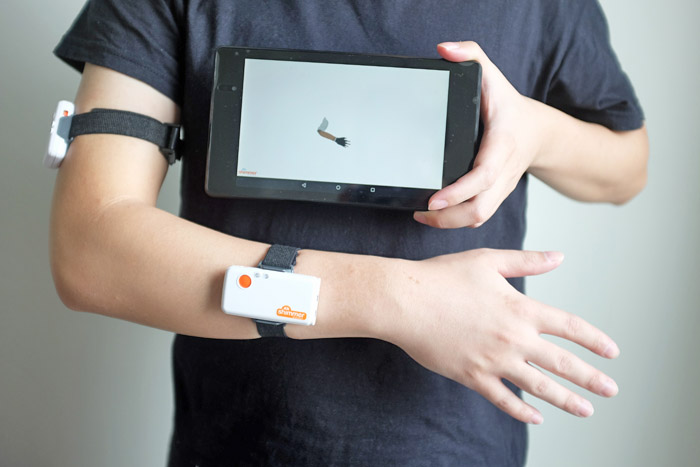
\includegraphics[scale=0.25]{Figures/Shimmer.jpg}
%  \caption{Wearable devices from the Shimmer platform.}
%  \label{fig:Shimmer}
%  \vspace{-0.3cm}
%\end{figure}
%
%
%All results collected and analyzed in this paper were obtained based on the energy consumption of wireless wearable devices (nodes), model 2R, produced by the company Shimmer~\cite{burns2010shimmer}. These instruments provide the collection of vital signs of patients through sensors, such as accelerometer, magnetometer, gyroscope, among others. Once collected, vital signs should be transferred to other more efficiently computational devices known as wireless body network coordinators. This transmission can be performed in two ways. The first one takes place directly, using Bluetooth technology. While the other mode would be with the aid of retransmission devices using ZigBee radio, since they provide better energy efficiency. 
%
%Os softwares que desenvolvemos para emular o monitoramento de sinais vitais, aplicados aos nós sensores Shimmer foram projetados com auxílio da linguagem de programação NesC~\cite{gay2014nesc}, a qual é baseada na linguagem C. Esta também é a linguagem adotada para o desenvolvimento do RTOS ({\em Real Time Operating System}), utilizado pelos nós sensores, e pelo Tinyos~\cite{levis2005tinyos}, o qual é um sistema operacional completamente voltado para aplicações em sistemas embarcados, permitindo a criação e a extensão de componentes específicos para cada característica de nó sensor.
%
%The NesC programming language is the basis for software development to these devices and for the RTOS (Real Time Operating System) running 
%Devices rely on a software developed in NesC programming language to %emulate the
%monitor vital signs. % applied to Shimmer sensor nodes was designed with the programming language NesC~\cite{gay2014nesc}, which is based on the C language. 
%NesC is also the basis for the %This is also the programming  language adopted for the 
%development of the RTOS (Real Time Operating System) running %on the wearable devices 
%together to TinyOS, %~\cite{levis2005tinyos},
%which is an operating system completely geared towards applications in embedded systems, allowing the creation and extension of components specific for each wearable device feature.


Energy consumption is measured in three different states (i.e., idle, sleep and run). At a glance, we set up the wearable to the desired state and continuously monitor it. The wearable device is automatically placed in a low-power mode when the task queue is empty (\textit{idle}: state 1). We can manually adjust the microprocessor for sleep mode (\textit{sleep}: state 2). In this sense, we are able to measure the wearable device lower level of power consumption. Finally, to monitor the wearable device on run state, we setup device to continuously perform a cryptography task ---on 64-bits data blocks--- using one of the aforementioned cryptography algorithms, followed by the encrypted data transmission using ZigBee (run: state 3) or Bluetooth (run: state 4).
Finally, unless we tell otherwise, at each state we perform 2000 samples and present mean confidence interval (for 95\% confidence level).


\begin{figure}[tbh]
 %\vspace{-0.3cm}
  \centering
  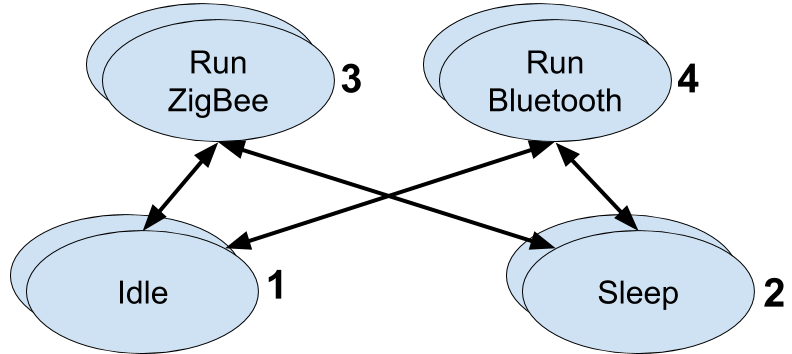
\includegraphics[scale=0.19]{Figures/estados.png}
  \caption{Wearable device states}
  \label{fig:states}
  \vspace{-0.1cm}
\end{figure}

We have designed and assembled a circuit for energy consumption measurement adapted from~\cite{bessa2017jetsonleap}. The circuit comprises of a low cost data acquisition board\footnote{DAQ - ADALM1000} connected to a wearable device, a 0.10~\si{\ohm} resistor, and a computer (Figure~\ref{fig:circuit}).
We use Active Learning Interface for Circuits and Electronics (ALICE) software to acquire voltage measurements from both terminals of the resistor which are connected to channels CH\_A and CH\_B of the DAQ. The voltage can be easily transformed to current following the law of Ohm, $V = R$ x $I$, since the resistance value is known. In order to make comparisons possible, we finally calculate the power consumption by multiplying the current to the voltage. Then, power consumption follows: 
$P = ((\mbox{CH\_A} - \mbox{CH\_B}) / 0.10) * V $ mW.



\begin{figure}[!htb]
 \vspace{-0.1cm}
  \centering
  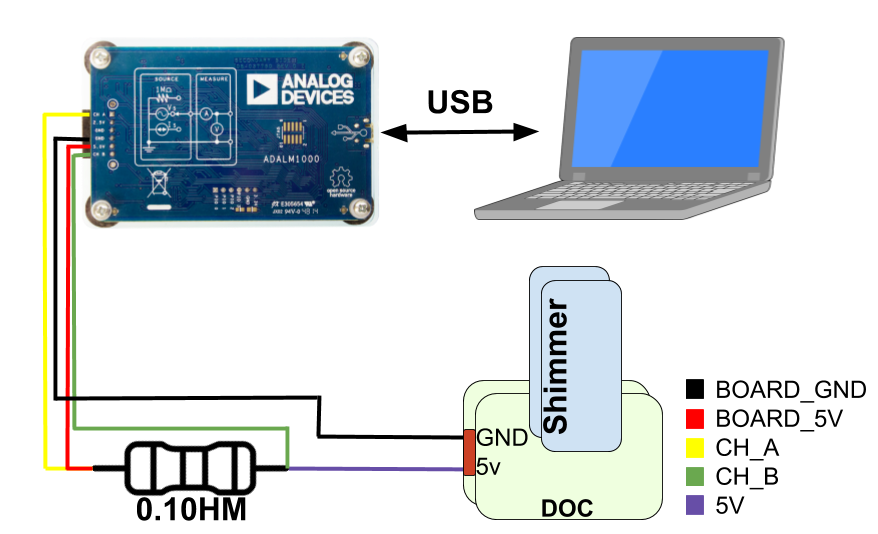
\includegraphics[scale=0.19]{Figures/circuit.png}
  \caption{Energy consumption measurement}
  \label{fig:circuit}
  %\vspace{-0.3cm}
\end{figure}

DAQ delivers a maximum sampling rate of 100 ksps (kilosamples per second).
 Therefore, we 
calculate energy consumption, mean, and the total consumption time for the algorithms in each analyzed state of wearable devices. Also, the computational complexity of the algorithms is of great relevance because energy consumption bottlenecks occur during data processing and transmission. Hence,  We also consider 
the size of machine code, since this represents a large share of the hardware resource consumption.


In addition to energy consumption, we analyze the main operations in each cryptography algorithm.
Hence, we
enumerate all the logical and arithmetic operations, once we want to confirm if the number of operations can be directly correlated with the final performance and energy consumption for the implementation of each algorithm.
Further, since wearable devices are severely constrained in computational resources, we also analyze the amount of memory the implementation of each algorithm consumes. We extract this information with the help of the NesC compiler.

